\documentclass{standalone}
\usepackage{pgfplots}
\usepackage{amsmath}
\usepackage{tikz}
\usetikzlibrary{patterns}
\usetikzlibrary{arrows.meta}

\begin{document}

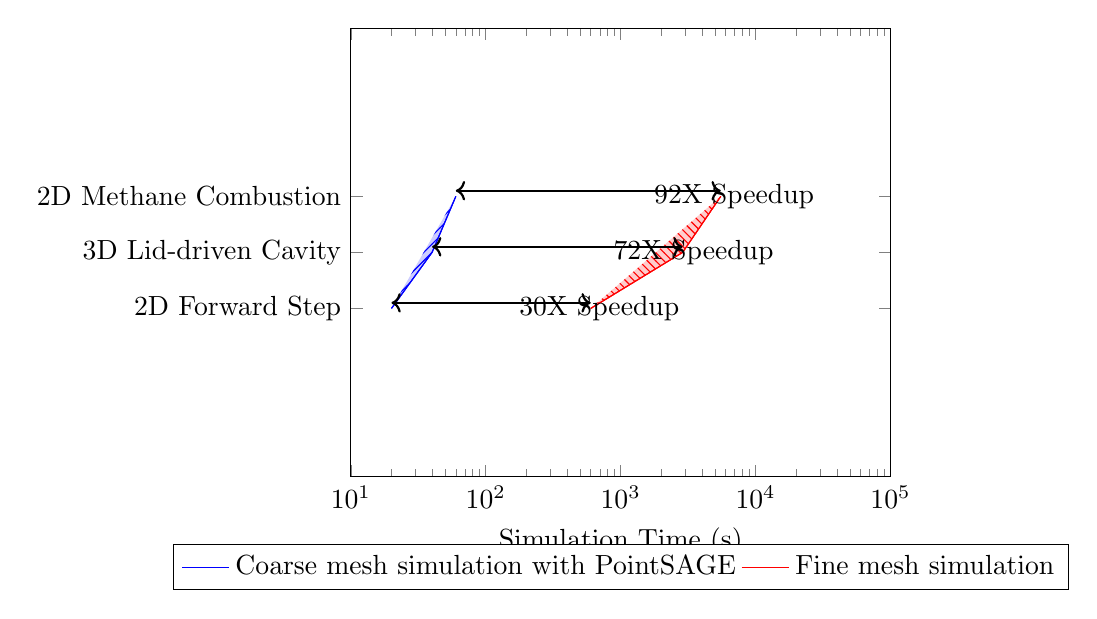
\begin{tikzpicture}
    \begin{axis}[
        xmode=log,
        xmin=10, xmax=100000,
        ymin=0, ymax=4,
        ytick={1, 2, 3},
        yticklabels={
            {2D Forward Step},
            {3D Lid-driven Cavity},
            {2D Methane Combustion}
        },
        xlabel={Simulation Time (s)},
        bar width=12pt,
        enlarge y limits=0.5,
        legend style={at={(0.5,-0.15)}, anchor=north, legend columns=-1},
        legend cell align={left}
    ]
    \addplot [
        draw=blue,
        fill=blue,
        fill opacity=0.2,
        postaction={
            pattern=north east lines,
            pattern color=blue
        }
    ] coordinates {(20,1) (40,2) (60,3)};
    
    \addplot [
        draw=red,
        fill=red,
        fill opacity=0.2,
        postaction={
            pattern=north west lines,
            pattern color=red
        }
    ] coordinates {(600,1) (2880,2) (5520,3)};
    
    \node[anchor=west] at (axis cs:150,1) {30X Speedup};
    \node[anchor=west] at (axis cs:750,2) {72X Speedup};
    \node[anchor=west] at (axis cs:1500,3) {92X Speedup};

    \draw[<->, thick] (axis cs:20,1.1) -- (axis cs:600,1.1);
    \draw[<->, thick] (axis cs:40,2.1) -- (axis cs:2880,2.1);
    \draw[<->, thick] (axis cs:60,3.1) -- (axis cs:5520,3.1);

    \legend{Coarse mesh simulation with PointSAGE, Fine mesh simulation}
    \end{axis}
\end{tikzpicture}

\end{document}